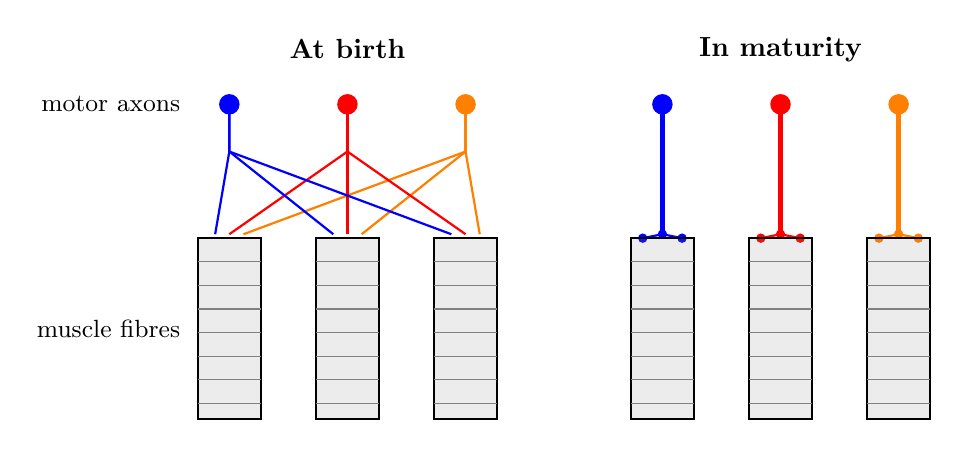
\begin{tikzpicture}[font=\small]
% ---------- AT BIRTH ----------
\node[font=\bfseries] at (1.5,4.3) {At birth};
% motor axons (cell bodies at top)
\fill[blue] (0,3.6) circle (0.13);
\fill[red] (1.5,3.6) circle (0.13);
\fill[orange] (3,3.6) circle (0.13);
% each axon branches to all three fibres
\foreach \tx in {0,1.5,3} {
  \draw[blue, thick] (0,3.6) -- (0,3.0) -- (\tx-0.18,1.95);
  \draw[red, thick] (1.5,3.6) -- (1.5,3.0) -- (\tx,1.95);
  \draw[orange, thick] (3,3.6) -- (3,3.0) -- (\tx+0.18,1.95);
}
% muscle fibres
\foreach \fx in {0,1.5,3} {
  \draw[thick, fill=gray, fill opacity=0.15] (\fx-0.4,-0.4) rectangle (\fx+0.4,1.9);
  \foreach \yy in {-0.2,0.1,...,1.7} {\draw[gray] (\fx-0.4,\yy) -- (\fx+0.4,\yy);}
}
% ---------- IN MATURITY ----------
\begin{scope}[shift={(5.5,0)}]
\node[font=\bfseries] at (1.5,4.3) {In maturity};
\fill[blue] (0,3.6) circle (0.13);
\fill[red] (1.5,3.6) circle (0.13);
\fill[orange] (3,3.6) circle (0.13);
\draw[blue, line width=1.6pt] (0,3.6) -- (0,1.95);
\draw[red, line width=1.6pt] (1.5,3.6) -- (1.5,1.95);
\draw[orange, line width=1.6pt] (3,3.6) -- (3,1.95);
% elaborated single endings
\foreach \fx/\c in {0/blue,1.5/red,3/orange} {
  \draw[\c, thick] (\fx,1.95) -- (\fx-0.25,1.9);
  \draw[\c, thick] (\fx,1.95) -- (\fx+0.25,1.9);
  \fill[\c] (\fx-0.25,1.9) circle (0.06);
  \fill[\c] (\fx+0.25,1.9) circle (0.06);
  \fill[\c] (\fx,1.95) circle (0.06);
}
\foreach \fx in {0,1.5,3} {
  \draw[thick, fill=gray, fill opacity=0.15] (\fx-0.4,-0.4) rectangle (\fx+0.4,1.9);
  \foreach \yy in {-0.2,0.1,...,1.7} {\draw[gray] (\fx-0.4,\yy) -- (\fx+0.4,\yy);}
}
\end{scope}
% shared labels
\node[left] at (-0.5,3.6) {motor axons};
\node[left] at (-0.5,0.75) {muscle fibres};
\end{tikzpicture}
